\section{Initial Database Architecture}
\subsection{High-Level Architecture Proposal}

\begin{figure}[H]
    \centering
    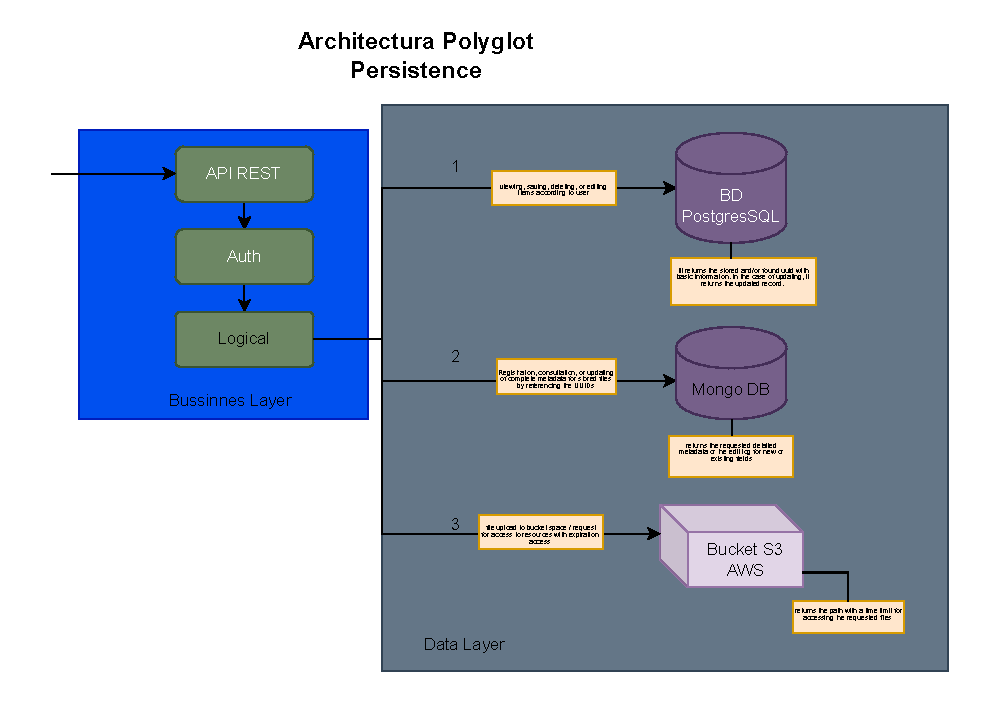
\includegraphics[width=\linewidth, height=0.4\textheight, keepaspectratio]{initialdbarch/architecture_diagram.pdf}
    \caption{Architecture High Level Model for the File Storage Platform.}
    \label{fig:architecture_diagram}
\end{figure}

\subsection{Entity Relationship Diagram - Second Version}
\begin{figure}[H]
    \centering
    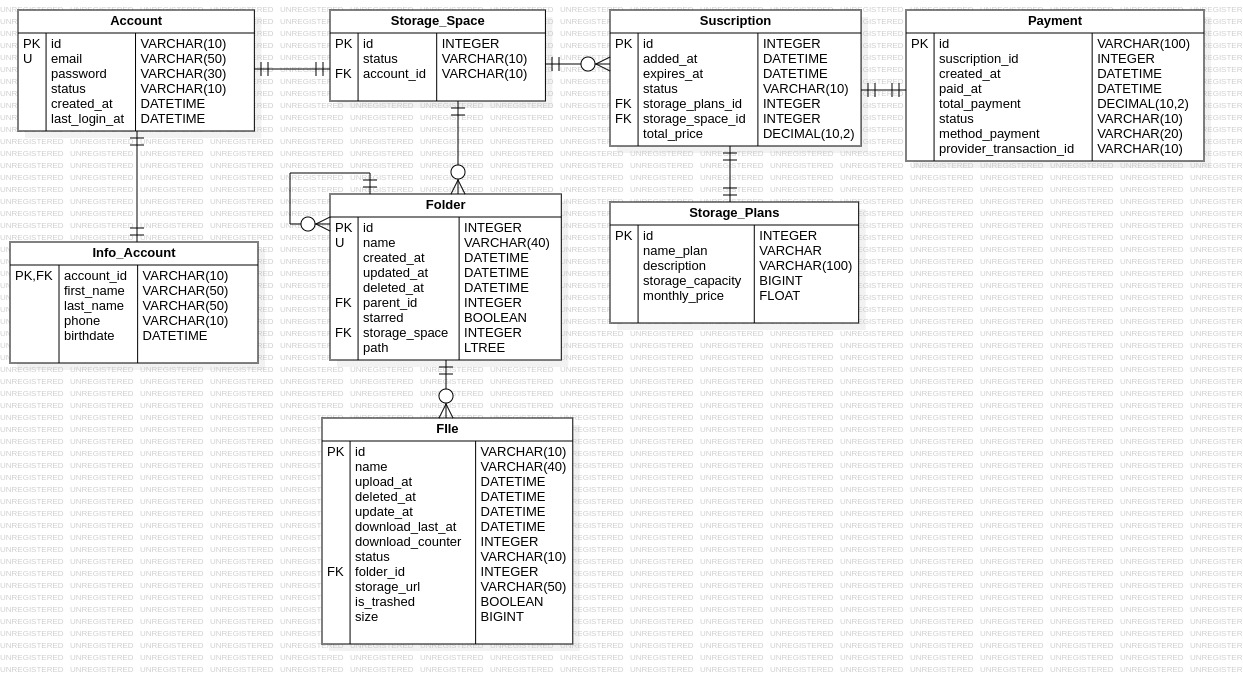
\includegraphics[width=\linewidth,height=0.95\textheight,keepaspectratio]{initialdbarch/ER.cloud.jpg}
    \caption{ First version of the entity relationship diagram for the file storage platform.}
    \label{fig:Entity Relaction}
\end{figure}
\textbf{NOTE: Considering the feedback on the need for deeper analysis and improved data storage design, it was decided to remove the metadata information from the relational model. All metadata variations will instead be managed within an unstructured data model. Therefore, the ER diagram includes only a superficial reference to the files, while detailed metadata will be stored at scale in the non-relational database, “MongoDB.” Furthermore, the use of the \textit{account → info\_account} relationship is justified by defining a mandatory one-to-one association, where each account must have exactly one corresponding account information record. Consequently, creating an account information record requires the presence of an existing account ID, as its primary key is a composite key that includes the account ID.}

\subsubsection{Description of entities}
\begin{itemize}
    \item The \textbf{Account} entity represents the user account within the system. It contains main fields such as \textit{id}, \textit{email}, \textit{password}, \textit{status}, \textit{created\_at}, and \textit{last\_access}. Its role is to be the starting point for all user information, since both personal settings and storage space are derived from it.

    \item \textbf{Info\_Account} complements the account with personal data: \textit{first\_name}, \textit{last\_name}, \textit{phone}, and \textit{birthdate}. It is directly associated with Account and serves to store user identification information.

    \item The \textbf{Storage\_Space} entity manages the storage space allocated to each account. It includes \textit{id}, \textit{status}, and a foreign key \textit{account\_id}. Its role is to serve as a link between the user and their storage subscriptions.

    \item \textbf{Subscription} stores the data for an active subscription: \textit{id}, \textit{added\_at}, \textit{expires\_at}, \textit{status}, \textit{total\_price}, along with references to the contracted plan and storage space. Its function is to record the conditions of use of the service for a given period.

    \item The \textbf{Payment} entity represents the payments made for a subscription. It contains \textit{id}, \textit{created\_at}, \textit{paid\_at}, \textit{total\_payment}, and \textit{method\_payment}. It allows you to keep track of the charges associated with each service contract.

    \item The \textbf{Folder} entity organizes files into hierarchies. Its most important fields are \textit{id}, \textit{name}, \textit{created\_at}, \textit{updated\_at}, \textit{deleted\_at}, \textit{parent\_id}, and \textit{starred}. It represents directories that can contain files and subfolders.

    \item \textbf{File} stores user file information. It includes \textit{id}, \textit{name}, \textit{created\_at}, \textit{deleted\_at}, \textit{download\_counter}, \textit{size}, and \textit{folder\_id}. It is responsible for representing the digital content within the folders.

    \item The \textbf{Format\_File} entity describes the file format. It contains \textit{name}, \textit{description}, and \textit{extension}. Its function is to identify the file type and its basic characteristics.

    \item Finally, \textbf{Metadata} complements the file with specific information such as \textit{mime\_type}, \textit{title}, \textit{author}, \textit{storage\_backend}, and \textit{complete\_metadata}. It serves to expand the technical and descriptive details of each file.
\end{itemize}
\subsubsection{Description of Relationships between Entities}
\begin{itemize}
    \item Account is related to Info\_Account, as each account has associated personal information.
    \item Account is linked to Storage\_Space, indicating the storage space allocated to each user.
    \item Storage\_Space is connected to Subscription, which defines the terms of the contracted service.
    \item Subscription is associated with Payment, which allows the payments for each subscription to be recorded.
    \item Folder is organized hierarchically by its parent\_id, and in turn contains multiple Files.
    \item File is related to Format\_File, to define the file type, and to Metadata, which expands its descriptive information.
\end{itemize}
\subsection{Data Flow and Storage Solutions}

The data architecture of the proposed file storage system focuses on how information is generated, transferred, and stored throughout the platform. The goal is to ensure secure handling of user data and efficient management of file storage while maintaining scalability and reliability. Figure~\ref{fig:Dataflow} illustrates the overall information flow.

\subsubsection{Data Flow}

When a user performs an operation such as registration, login, or file upload, the system validates the request and processes the corresponding data transaction. 
During authentication, user credentials are verified against the database, and secure session identifiers are generated.  
In file upload operations, the file’s binary content and descriptive metadata are separated:  
\begin{itemize}
    \item The \textbf{binary content} is stored directly in a cloud-based object storage service.
    \item The \textbf{metadata} name, size, type, upload date, and owner is recorded in the relational database.
\end{itemize}

For retrieval or download requests, metadata is used to locate the file in storage, and a temporary access token or signed URL ensures that only authorized users can retrieve it.  
All user interactions—such as upload, deletion, or access—are recorded in activity logs that support traceability and auditing.  

This structure ensures a clear distinction between operational data, transactions and sessions and persistent data, files and metadata, simplifying future scalability and maintenance.

\subsubsection{Storage Solutions}

The system uses a hybrid data storage model that separates structured and unstructured data for efficiency and flexibility.

\begin{itemize}
    \item \textbf{Relational Database PostgreSQL.}  
    Stores user information, permissions, and file metadata. The relational model ensures consistency, supports indexing, and facilitates query optimization.

    \item \textbf{Object Storage S3-compatible.}  
    Handles unstructured binary data, storing files using unique identifiers linked to metadata entries. This provides scalable and cost-effective storage for large files.

    \item \textbf{Cache Redis, optional.}  
    Temporarily stores frequently accessed metadata to improve query response times and reduce database load.

    \item \textbf{Logging and Backup.}  
    The system maintains logs for user actions and performs periodic backups of metadata and configuration data to support recoverability and auditing.
\end{itemize}

This architecture allows for secure, modular, and efficient data handling while remaining lightweight and scalable for a prototype implementation.

\begin{figure}[H]
    \centering
    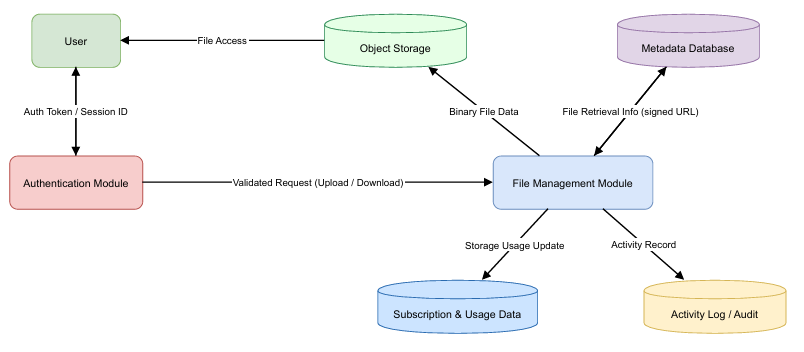
\includegraphics[width=0.9\linewidth,keepaspectratio]{initialdbarch/DataFlow.png}
    \caption{Data Flow and Storage Logic of the file storage platform.}
    \label{fig:Dataflow}
\end{figure}

The proposed data flow and storage logic establish a clear separation between user interaction data, operational transactions, and persistent storage. By isolating metadata management from binary file handling, the system ensures scalability, integrity, and efficient retrieval of information. The hybrid storage model—combining relational databases and object storage—provides flexibility for future growth while maintaining a lightweight implementation suitable for a prototype environment.
